\chapter{Metodologia}
\label{sec:metod}

\section{Camada de Rede}
A primeira etapa da construção da infraestrutura consiste na criação de uma VPC (Virtual Private Cloud), que representa uma rede virtual logicamente isolada dentro da AWS. Em seguida, são criadas as sub-redes (\textit{subnets}), cada uma associada a uma \textit{Availability Zone} (AZ), permitindo a distribuição dos recursos em diferentes zonas físicas dentro da mesma região, o que contribui para a resiliência da arquitetura.

\subsection{Entrada/saída e Gateways}
Para permitir o acesso à internet, é necessário criar um \textit{Internet Gateway} (IGW) e vinculá-lo à VPC. Sem essa associação, os recursos implantados não possuem conectividade externa.

\section{Camada de Aplicação}
Na camada de aplicação deste projeto, optou-se pela utilização de contêineres em modo \textit{Fargate}, em função de seu menor custo operacional e da facilidade de escalabilidade horizontal, características que o tornam ideal para aplicações com variação de carga \cite{redhat2024containers}.

\subsection{Conexão com o S3}
Para que nosso container acesse o armazenamento, ele precisaria de saída para a Internet, o que não é ideal. Por isso usamos o \textit{S3 Gateway Endpoint}: é mais barato que manter tráfego passando pelo NAT Gateway, é gerenciado pela AWS, altamente disponível por natureza e não exige IGW/NAT no caminho para o S3\cite{awsendpoint}.


\subsection{Balanceamento com ALB}
Para garantir o balanceamento de carga entre as tarefas em execução, foi implementado um \textit{Application Load Balancer} (ALB). Durante sua configuração, o ALB é associado a sub-redes públicas em múltiplas \textit{Availability Zones}, permitindo que opere de forma redundante em diferentes localidades dentro da mesma região. Essa abordagem proporciona tolerância a falhas e alta disponibilidade, assegurando a continuidade do serviço mesmo em caso de falhas parciais da infraestrutura \cite{aws2024alb}.

\subsection{Sessão e Stickiness}
Na camada de aplicação, por se adotar um contêiner personalizado em sub-redes privadas, utiliza-se um \textit{NAT Gateway} para o tráfego de saída. A persistência de sessão por \textit{Cookie Stickiness} no \textit{Application Load Balancer} é opcional e deve ser habilitada apenas quando a aplicação exigir afinidade para manter sessões autenticadas. Em cenários sem autenticação (login), tal configuração não se faz necessária.

\subsection{Identidade e Acesso (IAM Roles)}
Neste projeto, serão utilizadas \textit{IAM Roles} (funções) para permitir que os serviços em execução na infraestrutura, como os contêineres hospedados no ECS Fargate, tenham acesso controlado a outros recursos da AWS. Com essa abordagem, nós permite baixar a imagem do container e salvar as imagens no nosso S3.

Essa arquitetura também responde à escassez de endereços IPv4 disponíveis globalmente. Ao centralizar as requisições externas por meio do NAT Gateway, é possível fazer com que múltiplos recursos da VPC utilizem apenas um único IP público, otimizando o uso de endereços, simplificando a configuração de rede e reduzindo custos operacionais.

Por fim, o NAT Gateway é associado a uma sub-rede pública e atua como um componente essencial para balancear segurança, escalabilidade e conectividade.\cite{aws2024nat}


As etapas descritas anteriormente, como a criação da VPC, sub-redes públicas e privadas, Internet Gateway, NAT Gateway e a configuração do contêiner em uma subnet privada, resultam na arquitetura representada na Figura~\ref{fig:vpc-simples}. Essa estrutura ilustra a comunicação do contêiner com a internet por meio de um NAT Gateway alocado em uma subnet pública, reforçando a separação lógica entre os componentes e garantindo maior segurança e escalabilidade no ambiente construído.

\begin{figure}[H]
\centering
\caption{Arquitetura da VPC com container acessando a internet via NAT Gateway}
\label{fig:vpc-simples}
\fbox{
   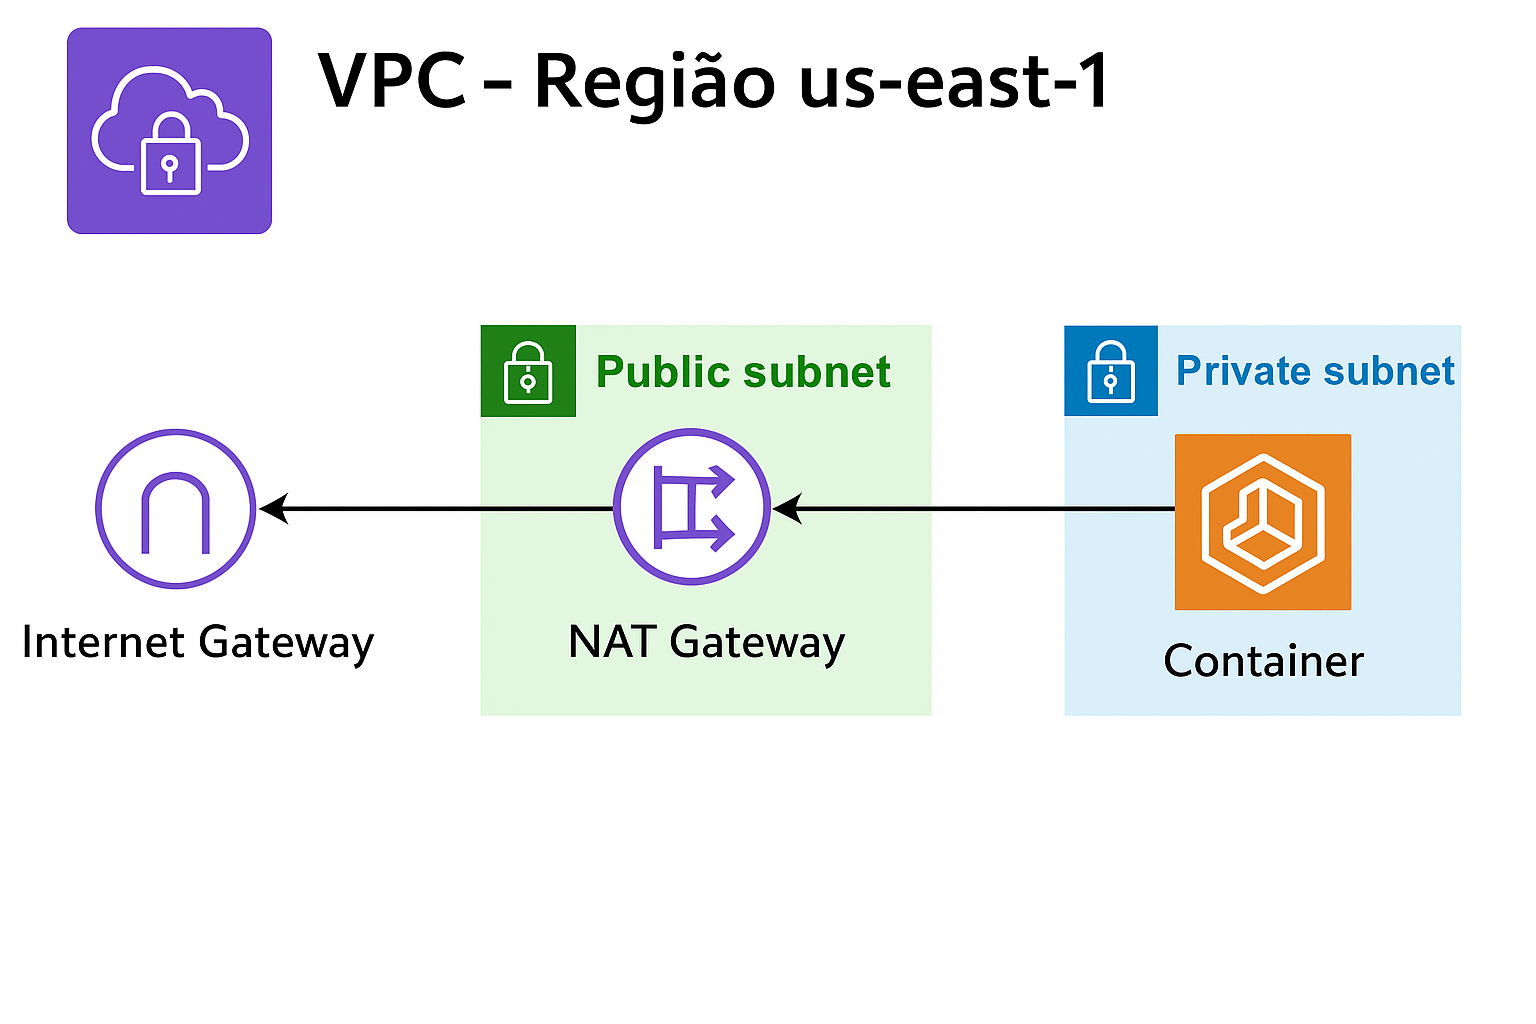
\includegraphics[scale=0.27]{imagens/vpc-simples.png}
}
\legend{Representação da infraestrutura configurada na AWS: o container, alocado em uma subnet privada, acessa a internet por meio de um NAT Gateway posicionado em uma subnet pública.}
\end{figure}


Para garantir a segurança da VPC, é necessária a utilização combinada de Security Groups e Network ACLs (NACLs). Os Security Groups atuam como firewalls com estado, sendo aplicados diretamente às instâncias e permitindo controlar o tráfego de entrada e saída com base em regras dinâmicas. Uma das funcionalidades mais vantajosas dos Security Groups é a possibilidade de fazer referência a outros Security Groups, permitindo que somente instâncias pertencentes a determinados grupos possam se comunicar entre si. Esse recurso facilita a escalabilidade e a gestão centralizada dos acessos na infraestrutura \cite{aws2024securitygroups}.

\subsection{Banco de Dados Gerenciado}\label{sec:metod-rds}
No contexto deste projeto, o banco de dados será acessado a partir do nosso container próprio, por meio de um usuário autenticado com login e senha específicos. Sendo assim, o banco de dados necessita apenas de uma regra de entrada em seu Security Group, permitindo conexões oriundas da aplicação. Todo o controle de autenticação será feito internamente pelo mecanismo de gerenciamento do banco, reforçando a segurança do acesso.

Para garantir alta disponibilidade e evitar pontos únicos de falha na arquitetura, é fundamental distribuir os recursos entre diferentes \textit{Availability Zones} (AZs) dentro de uma mesma região da AWS. Essa abordagem assegura que, caso uma AZ enfrente problemas, as demais possam manter o funcionamento dos serviços, proporcionando resiliência ao sistema.

\subsection{Armazenamento de Objetos}\label{sec:metod-s3}
Embora a resiliência entre regiões (\textit{cross-region}) envolva a replicação de toda a arquitetura em outra região geográfica, o foco deste projeto está na resiliência entre AZs, que oferece um equilíbrio entre disponibilidade e complexidade operacional.

Alguns serviços da AWS são projetados para serem resilientes por padrão. Por exemplo, o \textit{Amazon S3} armazena dados de forma redundante em múltiplas AZs, garantindo alta durabilidade e disponibilidade \cite{netapp2024ha}.

Apesar de o S3 “aparecer” na nossa \textit{região}, ele \textbf{não fica dentro da nossa VPC}. O S3 é um serviço regional da AWS exposto por endpoints públicos, a AWS basicamente “injeta” o serviço na região, mas o bucket não tem IP/ENI na VPC. 

Por isso usamos o VPC Gateway Endpoint, ele cria um alvo lógico nas nossas \textit{route tables} privadas e desvia o tráfego pro S3 por um caminho \textbf{privado}, gerenciado e possuindo alta disponibilidade. 

No entanto, outros serviços requerem configurações específicas para alcançar alta disponibilidade:

\begin{itemize}
  \item \textbf{Amazon RDS}: Para bancos de dados relacionais, é recomendada a implantação \textit{Multi-AZ}, onde uma instância primária é replicada de forma síncrona para uma instância em espera em outra AZ. Em caso de falha, o RDS realiza automaticamente o \textit{failover} para a instância secundária \cite{aws2024rds}.
  
  \item \textbf{Amazon ECS (Fargate)}: Ao utilizar o ECS com Fargate, é possível distribuir as tarefas entre múltiplas AZs, aumentando a resiliência da aplicação.
  
  \item \textbf{NAT Gateway}: Para permitir que instâncias em sub-redes privadas acessem a internet, recomenda-se a criação de um NAT Gateway em cada AZ utilizada, evitando dependência de uma única zona e melhorando a disponibilidade \cite{aws2024nat}.
\end{itemize}

\subsection{Arquitetura Geral em 3 Camadas}\label{sec:metod-fig-geral}
Ao adotar essas práticas, a arquitetura do projeto se torna mais robusta e preparada para lidar com falhas em componentes individuais ou em AZs inteiras, garantindo a continuidade dos serviços e a integridade dos dados.

A Figura~\ref{fig:arquitetura-geral}, a seguir apresenta a arquitetura planejada para o projeto, organizada em três camadas distintas: Camada de Balanceamento, Camada de Aplicação e Camada de Banco de Dados. Cada camada está distribuída entre duas sub-redes (Subnet A e Subnet B), refletindo uma estratégia de alta disponibilidade entre Zonas de Disponibilidade (AZs). Essa abordagem garante resiliência e escalabilidade da solução implementada.

\begin{figure}[H]
\centering
\caption{Arquitetura geral do ambiente na AWS}
\label{fig:arquitetura-geral}
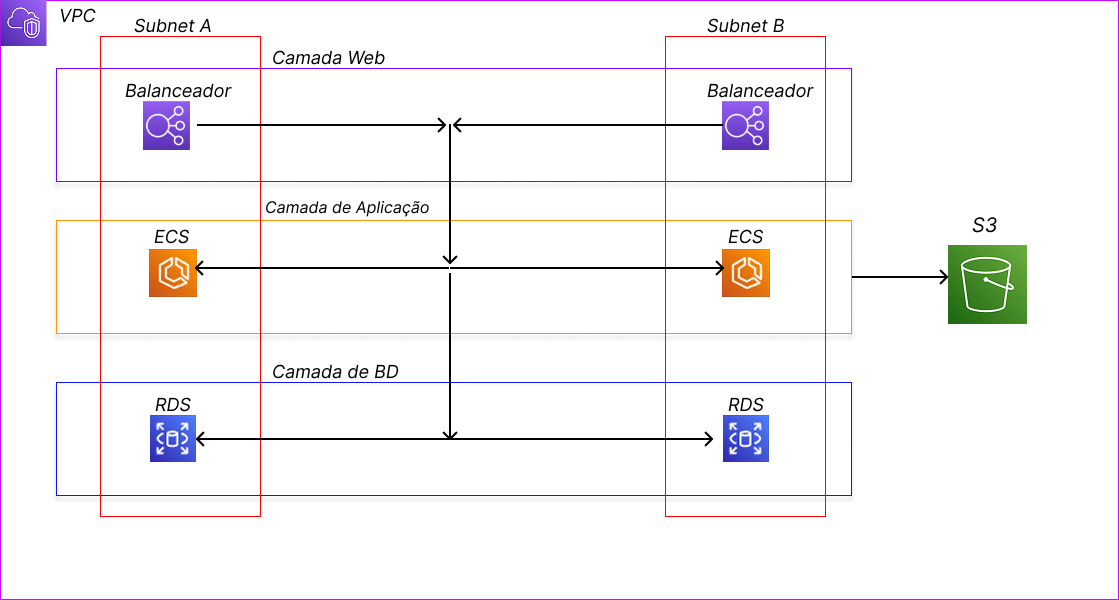
\includegraphics[scale=0.4]{imagens/arquitetura.png}
\legend{Visão em camadas da infraestrutura: balanceamento, aplicação e banco de dados, com distribuição entre duas sub-redes em Zonas de Disponibilidade distintas.}
\end{figure}


Na AWS, a principal ferramenta para implementação de IaC é o \textit{AWS CloudFormation}, que permite descrever toda a infraestrutura em arquivos escritos nos formatos JSON ou YAML. No contexto deste projeto, optou-se pela utilização do formato YAML por sua legibilidade e simplicidade sintática, o que facilita a manutenção e compreensão do código de infraestrutura.\cite{aws2024cloudformation}

Com essa abordagem, todos os recursos utilizados, como VPCs, sub-redes, gateways, grupos de segurança, serviços ECS, RDS e S3, são declarados em um único arquivo, possibilitando o controle de versão, repetibilidade e automação do ambiente de nuvem.


